\chapter{INTRODUCTION}\label{chapter:introduction}

Computer programs are full of faults. Faults cause programs to misbehave, work slowly and leak data. Even though it would be desirable that programs would work perfectly, prior studies have shown that this is not practical or impossible to achieve due to the inherent complexity of the programs and related aspects \cite{simmonds2018complexity,weinberg2008perfect,glenford2012art}. Thus software testing is fighting against programming faults and can be seen as an evergreen subject. Software testing has evolved over the years, but there is still much to be researched \cite{glenford2012art}. One of the areas of software testing is automated testing, which is often used for fighting against faults. In this thesis, a new regression test automation system is invented for the M-Files' Hubshare software.

Based on Google Scholar's 22 500 hits for the exact query "Test automation", it can be stated that generally, test automation has been studied extensively \cite{googleScholar}. Due to the sheer amount of papers, research is highly varied. According to Garousi and Mäntylä study, model-based testing methods, web services-based software, and regression testing are currently the most popular aspects in their respective categories \cite{garousi2016software}. Based on the Ricca et al. literature review \gls{ai} based test automation solutions have been proposed for common problems like resources it takes to develop test automation, untested code, and extra maintenance overhead \cite{aiRicca2021}. As a solution, automated test generation, visual testing, and self-healing mechanisms have been provided \cite{aiRicca2021}. A checklist was assembled by Garousi and Mäntylä to support decision-making on whether to automate particular aspects of the \gls{sut} or not \cite{garousi2016when}. In their work, they identified that many aspects support automation, but things like upcoming major modifications, unpredictability and complexity decrease the feasibility of the test automation.

As stated in the previous paragraph, test automation has been researched rigorously, and multiple studies have been made about it. However, there has yet to be a comprehensive, in-depth case study about planning, developing and deploying full-scale industrial regression test automation solutions in a single white paper. There have been many comprehensive case studies about test automation, but all of them have been shallower case studies \cite{graham2012experiences} or in-depth, but laser-focused case studies \cite{garousi2018introducing,ramler2018adapting,lee2018architecture}. Nevertheless, there has not been a comprehensive, in-depth case study of a single system that covers the whole regression testing automation spectrum and related management matters as is provided in this thesis.

\section{Definition of the problem}
M-Files Hubshare is a file-sharing and intranet platform which has been in active development since 2013 \cite{mfiles2022Hubshare,hubshare2020}. Even though the platform has been in development for multiple years, its adoption of regression test automation has been minimal. Instead, manual regression testing has been used extensively to prevent regressions from occurring in releases. The issue with manual testing is that the testing is tedious and cannot be done as often as automated regression testing \cite{akin2018transitioning}, which restricts, for example, the phase of the releases. In addition, manual testing is always somewhat subjective due to human factors \cite{akin2018transitioning}. Manual testing exposes software for possible testing errors and thus regression defects \cite{garousi2016developing}.

Because of the previously mentioned issues, implementing regression test automation has been seen as a necessary activity in Hubshare's software development. However, this need raises multiple questions that must be resolved before the regression test automation system can be fully taken into daily use. How can different parts of the software be isolated using fakes so that the software can be tested in pieces? How are developers educated to write good automation test cases? In which way the daily test automation activities can be carried out effectively?

Since the problem is broad, only some of the questions can be answered in a single thesis. This thesis focuses on answering the following \glspl{rq}:
\begin{enumerate}[label=RQ\arabic*,noitemsep]
	\item\label{rq1} What management-related aspects must be considered regarding the test automation systems?
	\item\label{rq2} How can test automation effectively be taken into daily use?
	\item\label{rq3} How to design a usable, performant and stable regression test automation system in all three major testing levels (unit, integration and system)?
\end{enumerate}

\section{Goals and limitations}\label{section:goals_and_limitations}
This thesis aims to design an overall functional comprehensive regression test automation system. The thesis does not consider other use cases of test automation like automated performance, security or usability testing. Other test automation types are out of the scope of this thesis because they require significantly different technologies and techniques compared to regression test automation and are not directly related. Additionally, \gls{ci} is mainly ignored from the technical standpoint in this thesis. During the project, it was realised that a simple virtual machine \gls{ci} setup is sufficient until test automation has matured considerably more.

Even though during this thesis, soft values like motivation and developer education are identified as necessary activities, those subjects will only be touched on in this work. The thesis focuses mainly on the technical and management perspectives, and educational aspects would be too far off from the main points. During this thesis, those subjects were still somewhat addressed because, in reality addressing those aspects is necessary and ignoring them would have left the test automation system incomplete.

This thesis contains a considerable amount of plans and technical details. However, due to the project's sheer size, the test automation system's technical side was not fully completed nor taken into daily use before publishing this thesis. It would have been impossible to complete the amount of work required for a complete system with the usable resources and time. Even most people involved in the project doubted this much could be achieved during the given time frame. As illustrated in the \autoref{fig:practical_implementation_status} unit automation testing systems were finalised, \gls{api} automation testing system was mostly finalised, and component level integration testing, as well as system testing, were not finalised during the thesis. Only backend unit testing was fully taken into use during the thesis. Because the project is still ongoing during the publication of this thesis, only preliminary results based on the gathered knowledge and created technical solutions are reported in this paper.

\begin{figure}
	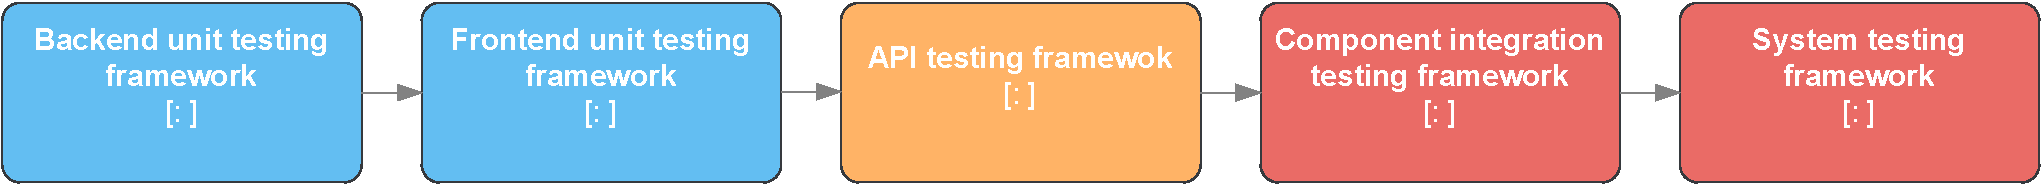
\includegraphics{Practical_implementation_status}
	\caption{Practical implementation's status at the publication time}
	\label{fig:practical_implementation_status}
\end{figure}
\FloatBarrier

\section{Structure of the thesis}
This thesis has eight primary chapters. During the \autoref{chapter:introduction}, thesis themes were introduced, and research questions were laid out. The literature review is conducted in the \autoref{chapter:background}, and the context of the project is described. Case and research methodologies are presented in the \autoref{chapter:case_and_research_methodologies}.

The first planning steps, information gathering, survey planning, and results, can be found in the \autoref{chapter:initial_planning_and_information_gathering}. In the \autoref{chapter:planning_of_the_test_automation_systems}, planning of the test automation systems will be described, including requirements, management and technical planning. During the \autoref{chapter:produced_test_automation_system}, the produced test automation system will be detailed, and its success will be evaluated based on the professional review's results. General discussion related to the project overall and specific aspects can be found in the \autoref{chapter:discussion}. Finally, conclusions are laid out in the \autoref{chapter:conclusions}.